% Options for packages loaded elsewhere
\PassOptionsToPackage{unicode}{hyperref}
\PassOptionsToPackage{hyphens}{url}
%
\documentclass[
  a4paper,
  11pt,
  twocolumn]{article}
\usepackage{amsmath,amssymb}
\usepackage{iftex}
\ifPDFTeX
  \usepackage[T1]{fontenc}
  \usepackage[utf8]{inputenc}
  \usepackage{textcomp} % provide euro and other symbols
\else % if luatex or xetex
  \usepackage{unicode-math} % this also loads fontspec
  \defaultfontfeatures{Scale=MatchLowercase}
  \defaultfontfeatures[\rmfamily]{Ligatures=TeX,Scale=1}
\fi
\usepackage{lmodern}
\ifPDFTeX\else
  % xetex/luatex font selection
\fi
% Use upquote if available, for straight quotes in verbatim environments
\IfFileExists{upquote.sty}{\usepackage{upquote}}{}
\IfFileExists{microtype.sty}{% use microtype if available
  \usepackage[]{microtype}
  \UseMicrotypeSet[protrusion]{basicmath} % disable protrusion for tt fonts
}{}
\makeatletter
\@ifundefined{KOMAClassName}{% if non-KOMA class
  \IfFileExists{parskip.sty}{%
    \usepackage{parskip}
  }{% else
    \setlength{\parindent}{0pt}
    \setlength{\parskip}{6pt plus 2pt minus 1pt}}
}{% if KOMA class
  \KOMAoptions{parskip=half}}
\makeatother
\usepackage{xcolor}
\usepackage{graphicx}
\makeatletter
\newsavebox\pandoc@box
\newcommand*\pandocbounded[1]{% scales image to fit in text height/width
  \sbox\pandoc@box{#1}%
  \Gscale@div\@tempa{\textheight}{\dimexpr\ht\pandoc@box+\dp\pandoc@box\relax}%
  \Gscale@div\@tempb{\linewidth}{\wd\pandoc@box}%
  \ifdim\@tempb\p@<\@tempa\p@\let\@tempa\@tempb\fi% select the smaller of both
  \ifdim\@tempa\p@<\p@\scalebox{\@tempa}{\usebox\pandoc@box}%
  \else\usebox{\pandoc@box}%
  \fi%
}
% Set default figure placement to htbp
\def\fps@figure{htbp}
\makeatother
\setlength{\emergencystretch}{3em} % prevent overfull lines
\providecommand{\tightlist}{%
  \setlength{\itemsep}{0pt}\setlength{\parskip}{0pt}}
\setcounter{secnumdepth}{5}
%------------------------------------------------------------------------------%
% PAPER TEMPLATE FOR ICPHS 2023 Prague                                         %
%                                                                              %
% Original template downloaded from:                                           %
% http://www.icphs2023.org/call-for-papers/                                    %
%                                                                              %
% Reformatted to work with Rmarkdown and R by:                                 %
% Joseph V. Casillas | Rutgers Univesity |11/11/2022                           %
%                                                                              %
% Available for download at:                                                   %
% https://github.com/jvcasillas/icphs2023_rmd_template                         %
%------------------------------------------------------------------------------%



% Packages
\usepackage{./includes/tex/icphs2023}
\usepackage{metalogo} 
\usepackage{epstopdf}
\usepackage{tipa}

% Links and urls must be black
%\hypersetup{urlcolor=black, citecolor=black, linkcolor=black}


% Packages removed from icphs2023.sty because of conflicts
% They have been added to the .Rmd yaml front matter
% \usepackage[latin1]{inputenc}
% \usepackage[T1]{fontenc}
% \usepackage[leqno,fleqn]{amsmath}
\usepackage[utf8]{inputenc}
\usepackage[T1]{fontenc}
\usepackage{bookmark}
\IfFileExists{xurl.sty}{\usepackage{xurl}}{} % add URL line breaks if available
\urlstyle{same}
\hypersetup{
  hidelinks,
  pdfcreator={LaTeX via pandoc}}

\author{}
\date{\vspace{-2.5em}}

\begin{document}

\title{Schwa to /a/: Development of Unstressed Vowels in L2 Spanish}
\author{Robert Esposito, Joseph V. Casillas}
\organization{Department of Spanish and Portuguese, Rutgers University}
\email{rme70@scarletmail.rutgers.edu, joseph.casillas@rutgers.edu}


\maketitle

\begin{abstract}
Native (L1) English second language (L2) Spanish learners acquiring the Spanish vowel system are tasked with adjusting entrenched vowel categories and morphophonological rules. For example, allophonic variation of stressed and unstressed vowels in English is not present in Spanish, but the triggering environments for the variation is present in Spanish. As such, learners of Spanish must come to ignore those triggering environments during perception and production. The present study examines the production of unstressed Spanish /a/ by 10 L1 English L2 Spanish learners during a seven-week domestic immersion program in a semi-longitudinal study. Preliminary acoustic analysis revealed that within the first week, participants fronted and lowered their production of unstressed /a/, assumed here to correspond to less centralization and more target-like production. The findings are situated within current models of second language speech learning and provide often-sought longitudinal data on an understudied phenomenon.
\end{abstract}

\keywords{phonetics, phonology, second language acquisition, Spanish, English}


\section{Introduction}

Adult native English (L1) learners of Spanish as a second language (L2)
face difficulties producing target-like Spanish vowels due to a
morphophonological centralization process in English in which unstressed
vowels tend to reduce categorically to a centralized vowel. For example,
a learner may produce the Spanish word /\textipa{"}ka.sa/ as
non-target-like {[}\textipa{"}ka.s\textipa{@}{]}. The present study
investigates the production of Spanish stressed and unstresed /a/ in 10
L1 English L2 Spanish beginner learners during a seven-week domestic
immersion program in a semi-longitudinal design. Instead of extracting
formant values at solely the midpoint of the vowel, acoustic analysis
includes a measure of vowel trajectory and spectral centroid to obtain a
more holistic view of vowel centralization. Results provide information
about typical development of L1 English L2 Spanish beginner learners
with growing L2 exposure and how learners adjust their production in the
face of growing evidence against a process present only in the L1.

\section{Literature Review}

\subsection{Spanish and English Vowels}

Reported variation in Spanish varieties should not be ignored in general
\cite{willis2005initial,lipski1994tracing,alba2006accounting}, but vowel
production has been found to be relatively uniform across varieties
\cite{tomas1957documentos,quilis1993tratado}, whereas descriptions of
English vowel systems vary more widely
\cite{ladefoged2006course,bradlow1995comparative}. Spanish can be said
to have a subset of English vowel phonemes /i e a o u/, but the phonetic
realizations of these phonemes are not identical.

A major difference to highlight between the two systems is the impact of
prosodic effects, such as lexical stress, on the realization of vowels.
One of the major acoustic correlates of lexical stress
cross-linguistically is vowel reduction in unstressed syllables
\cite{gordon2017acoustic}. Spanish has been found to have minimal
centralization of vowels in unstressed syllables
\cite{martinez1984fonetica,tomas1957documentos}, representing a possibly
universal low-level phonetic phenomenon \cite{kapatsinski2020vowel}. On
the other hand, English presents both low-level phonetic reduction like
Spanish, as well as a language-specific, morphophonologic, categorical,
rule-based process in which vowels in lexically unstressed syllables are
realized as centralized vowels \textipa{[I]} or \textipa{[@]}
\cite{bybee2003phonology,barnes2008strength,fourakis1991tempo}. For
example, the first vowel in the English word `atom' is realized as
\textipa{[\ae]} in the tonic syllable, but when realized in a non-tonic
syllable like in the derived word `atomic', the vowel is obligatorily
reduced to \textipa{[@]}.

\subsection{L1-L2 Transfer Effects}

L1 English L2 Spanish learners typically do not present major issues
acquiring phonological vowel contrasts \cite{morrison2003perception},
but the phonetic and morphophonological differences between their L1 and
L2 may result in non-target-like production
\cite{aldrich2014acquisition,cobb2009pronunciacion,cobb2015adult,iruela1997adquisicion,menke2010second}.
The acquisition path of Spanish vowels by L1 English L2 Spanish learners
can be accurately described by a number of frameworks such as the Speech
Learning Model revised \cite{flege2021revised}, the Perceptual
Assimilation Model \cite{best2007nonnative}, or, as will be explored
here, the Second Language Linguistic Perception (L2LP) model
\cite{escudero2004bridging,escudero2005linguistic,escudero2007second,escudero2009linguistic,van2015learning}.

The L2LP model proposes that L2 learners create a new grammar via
\emph{full copying/full access}. Accordingly, difficulties in acquiring
L2 speech sounds are accounted for by phonetic similarities,
differences, or perceived equivalences to contrasts present in the L1.
The learner must adjust their perception grammar to account for L2
input. Based on this framework, it is expected that linguistic processes
present in the L1 may undesirably surface in the L2, but that these
transfer effects may be reduced with increasing exposure to and
proficiency in the L2. For example, \cite{casillas2016longitudinal}
found that L1 English L2 Spanish late learners over a seven-week
home-immersion program shifted perception and production of voice onset
time categorical boundaries from initially English-like towards more
Spanish-like values.

As mentioned, English presents vowel allophony in lexically stressed and
unstressed positions not present in Spanish. In a cross-sectional study,
\cite{cobb2015adult} found that L1 English L2 Spanish late learners of
Spanish, divided into ``intermediate'' and ``advanced'' proficiency
groups, produced unstressed Spanish vowels as more centralized than L1
Spanish controls. Although valuable, \cite{escudero2005linguistic} urges
for the inclusion of longitudinal data from beginning language learners.
Longitudinal L2 acquisition data has provided evidence, for example,
that the formation of L2 phonetic categories can occur abruptly at early
stages \cite{casillas2020phonetic}.

\section{The Present Study}

In sum, previous research has pointed to the difficulties of L1 English
L2 Spanish target vowel production, particularly when it comes to
unstressed vowels due to L1-L2 transfer effects. Available studies
typically present cross-sectional designs. From an L2LP perspective,
cross-sectional designs only tell part of the story, and longitudinal
data will reveal how the L2 grammar is progressively adjusted as the
learner receives more input. As such, the present study tracks the
production of /a/ in stressed and unstressed position in 10 L1 English
L2 Spanish beginner late learners during a seven-week domestic immersion
program in a semi-longitudinal design. With this data, the following
research questions (RQs) are answered:

\begin{enumerate}
\item Do L1 English L2 Spanish learners centralize unstressed Spanish /a/?
\item Do L1 English L2 Spanish learners reduce centralization of unstressed Spanish /a/ as they progress through a 7-week domestic immersion program?
\end{enumerate}

Based on the L2LP
\cite{escudero2004bridging,escudero2005linguistic,escudero2007second,escudero2009linguistic,van2015learning},
it was predicted that learners will initially produce unstressed /a/ as
more schwa-like due to lexical stress effects present in the L1
\cite{bybee2003phonology,cobb2009pronunciacion,cobb2015adult}, but that
centralization would reduce over the seven-week period
\cite{casillas2016longitudinal}. Furthermore, as has been seen in
research on other segmentals \cite{casillas2020phonetic}, it is
hypothesized that participants will demonstrate abrupt, as opposed to
gradual, development in target-like production of unstressed /a/.

\section{Methodology}

\subsection{Participants}

Ten L1 English L2 Spanish late learners (6 females; ages 18--34 years,
\(\bar{x}\) = 23.7) were recruited for the present study. They reported
no prior experience with any foreign languages, nor had they spent a
significant amount of time in a foreign country. Participants were
enrolled in the Middlebury Spanish Language School program's beginner
classes, placed via a placement test and interviews with two faculty
members of the program. The Middlebury Language School program is a
seven-week domestic immersion program where students are encouraged and
quasi-obligated to use their target language at all times. During the
seven-week program, participants received high amounts of L2 input (from
native and non-native speakers) and reported minimal L1 use.

\subsection{Materials}

Participants completed a delayed repetition task during the first week,
and in subsequent weeks, a reading task. The analyzed materials
consisted of 18 real and nonce words. Each word was a bisyllabic
paroxytone with /a/ as the final vowel. While the first syllable
variably contained an onset, the second syllable always contained an
onset (e.g., ada, ita, gaka, gota). Auditory stimuli for the first week
was produced by a 29 year old L1 Spanish speaker from Cádiz, Spain, who
produced the words in a carrier phrase. Participants were recorded in a
quiet classroom on site at Middlebury College using a Shure SM10A
dynamic head-mounted microphone. A Sound Devices MM-1 pre-amplifier
boosted the signal and sent it to a laptop computer where it was
recorded using Praat at a 44.1 kHz sample rate with a 16-bit
quantization \cite{boersma2025praat}.

\subsection{Procedure}

Participants completed the first experimental session on the second or
third day of the program; further experimental sessions took place every
Sunday, for a total of 7 sessions. Stimuli were presented randomly to
participants using PsychoPy2 \cite{peirce2019psychopy2}, aurally for the
first session and visually in subsequent sessions. Participants listened
or read aloud each item 3 times. Each participant provided the dataset
with 378 items for a total of 3780 tokens (18 words * 3 repetitions * 7
weeks * 10 participants).

\subsection{Acoustic Analysis}

Recordings were transcribed, segmented automatically
\cite{mcauliffe2017montreal}, and manually corrected when necessary. A
Praat script \cite{vargo2025praat} was then used to extract formant
values at 10\% intervals of target vowels. A ``spectral centroid'' was
calculated by averaging formant values at equidistant points spanning
20\% to 80\% of the vowel, which present less coarticulatory effects
resulting from consonant environment
\cite{jacewicz2011vowel,coretta2024tutorial}. The trajectory length (TL)
of vowels was also calculated, which represents a measure of formant
movement \cite{fox2009cross}. Longer TL is associated with greater
formant movement: ``dipthongal'' vowels tend to have TLs that exceed 620
Hz, whereas ``dipthongized'' vowels fall between 420 and 620 Hz
\cite{jacewicz2011regional}.

\subsection{Statistical Analysis}

Generalized additive mixed models (GAMMs)
\cite{soskuthy2017generalised,coretta2025tutorial} were fit to F1 and F2
centroids, measured in Hertz (Hz), with a parametric term for the
variable \emph{stress} to model mean differences in Hz between stressed
and unstressed /a/. Smooth terms for \emph{session} and \emph{stress} by
\emph{session} were included to model non-linear effects of time for
stressed and unstressed vowels. Another GAMM was fit to trajectory
length (TL) with identical parametric and smooth terms. All three models
included a random factor smooth by subject over session was included to
model by-subject differences.

Models were interpreted using quantitative and visual methods
\cite{soskuthy2017generalised}. \emph{P}-values for the parametric
\emph{stress} term was evaluated at \(\alpha\) = 0.05 to determine if
there is a difference in overall mean Hz for stressed and unstressed
vowels for F1, F2, and TL. Visual inspection of the difference plots
were also used for the same comparison. Confidence intervals that do not
overlap with 0 were taken as evidence that the two estimates are
different. Lastly, F1, F2, and TL smooths were plotted to view their
trajectories over session for a more individual, fine-grained
inspection.

\section{Results}

For F1, F2, and TL, stress was a significant parametric predictor.
Stressed /a/ had higher F1 (\(\beta\) = , SE = ), lower F2 (\(\beta\) =
, SE = ), and shorter TL (\(\beta\) = , SE = ). None of the
population-level smooths reached significance for F1, F2, or TL. In
contrast, participant-specific session smooths were significant in all
three models (F1: EDF = 43.93, \(F\) = 206.26; F2: EDF = 42.1, \(F\) =
122.8; TL: EDF = 36.85, \(F\) = 66.93), indicating substantial
individual differences in trajectories for F1, F2, and TL across the
seven sessions.

\begin{figure}[!ht]
\begin{center}
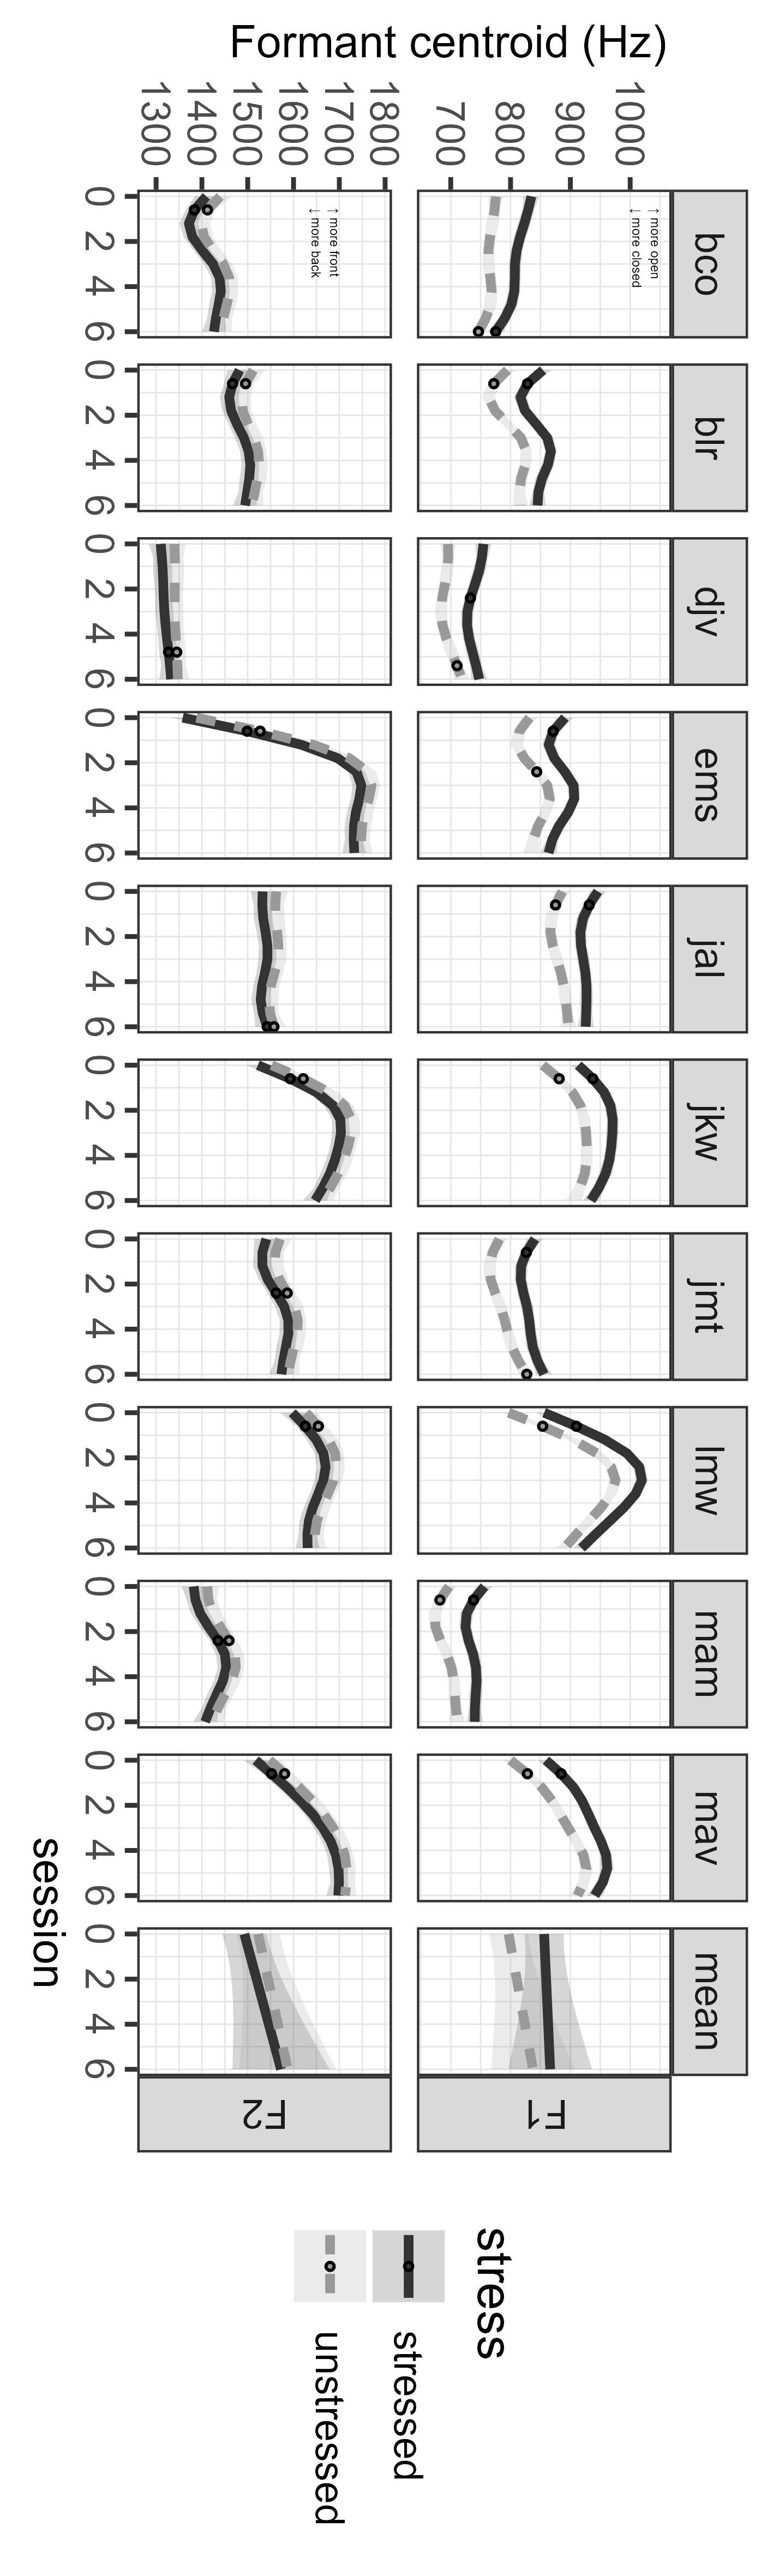
\includegraphics[width=6cm,height=20cm]{./includes/figures/f1_f2_p_all.png}
\caption{Individual and population-level (right-most panel) F1 and F2 trajectories for stressed and unstressed vowels over 7 weeks. The moment of largest absolute change is marked with a circle.}
\label{fig:f1-f2}
\end{center}
\end{figure}

Visual inspection of the population means \ref{fig:f1-f2} revealed that
the learners were ``closing the gap'' between stressed and unstressed
/a/ for F1 and F2, but difference plots (not printed here for lack of
space) revealed that the formant differences between stressed and
unstressed /a/ remained different from zero. For F1, stressed /a/ did
not change much over the weeks, but unstressed /a/ clearly rose over the
weeks to approach values similar to stressed /a/, indicating that their
unstressed /a/ production became more open. For F2, unstressed and
stressed /a/ values were similar from the beginning and presented
similar upward movement, indicating that /a/ production became more
fronted. For F2, unstressed and stressed /a/ similarly sloped upward
across time, indicating that /a/ productions became more fronted.

\section{Discussion}

The present work examined the production of /a/ in L1 English L2 Spanish
beginner learners in a domestic immersion program in a semi-longitudinal
design. Based on L2LP
\cite{escudero2004bridging,escudero2005linguistic,escudero2007second,escudero2009linguistic,van2015learning},
it was expected that these learners would present centralization of
unstressed /a/ due to L1-L2 transfer
\cite{bybee2003phonology,cobb2009pronunciacion,cobb2015adult}, but
transfer effects would be mitigated with increasing L2 proficiency and
exposure. In line with previous work, it was found that stressed and
unstressed /a/ production differed in F1 and F2 at all time points. This
is not particularly surprising, as even native Spanish controls and
``advanced'' learners presented slightly centered productions of
unstressed /a/ compared to stressed /a/, although the two categories
heavily overlapped \cite{cobb2015adult}. Importantly, F1 values for
stressed and unstressed /a/ became more and more similar across the
seven weeks, with unstressed /a/'s F1 raising while stressed /a/
maintained similar values, evidence for less centralization. The lack of
movement for F1 in stressed /a/ is in line with previous work that
indicates that F1 values for English and Spanish /a/ in CVCV syllables
are similar \cite{bradlow1995comparative}. F2 values for stressed and
unstressed /a/ both became higher across the seven weeks, indicating
that the learners were fronting their /a/ more, in line with previous
work identifying Spanish /a/ as more fronted than English /a/
\cite{bradlow1995comparative}. Although the F2 difference plot showed a
downward slope, there was not strong evidence that F2 was becoming
closer for stressed and unstressed /a/.

Although /a/ productions were changed, there is no clear evidence from
grand mean values that the changes were abrupt
\cite{casillas2020phonetic}. In fact, the GAMMs reports a linear,
gradual change to F1 and F2 values across the weeks. Examining each
participant's smooths \ref{fig:f1-f2}, however, reveals that the moment
of greatest absolute change in F1 or F2 for each stressed and unstressed
/a/ occurred, in most cases, early.

\section{Limitations and Future Direction}

There a number of improvements that can be made to the current study.
First, the current data analyzed only /a/, which may show a different
development pattern than other vowels \cite{cobb2015adult}. Trajectory
length, for example, may prove to be a more useful measure of
development for mid vowel production, which are typically diphthongized
in English and transferred to Spanish. In terms of perception, the L2LP
posits that perception precedes production \cite{escudero2007second},
but the current data cannot provide evidence on this topic. In a case
like this, perceptual boundaries of /a/ versus \textipa{/@/} could be
investigated in L1 English L2 Spanish learners
\cite{miller1989auditory}. Lastly, accurate vowel categorization bears
morphological weight in Spanish: centralized vowels may result in
inaccurate perception or production of gender or verb morphology. As
such, future investigations should examine vowel acquisition vis-a-vis
morphological acquisition.

\section{Conclusion}

The present study analyzed the production of unstressed /a/ in 10 L1
English L2 Spanish beginner learners in a domestic immersion program in
a semi-longitudinal design over seven weeks. Learners' stressed and
unstressed /a/ productions became more similar across the seven weeks,
and their F2 values became more target-like. This study deepens our
understanding of how L1 morphophonological processes not present in the
L2 may arise in L2 production and provides evidence for rapid
development of fine-grained phonetics early in exposure to an L2.

\subsection{References}

\bibliographystyle{./includes/bib/IEEEtran.bst}
\bibliography{./includes/bib/icphs2023.bib}

\theendnotes

\end{document}
